% Условная компиляция для самостоятельной работы
\ifdefined\mainfile
    % Если это часть основного файла, не добавляем начало и конец документа
\else
    \documentclass[12pt, a4paper]{report}
    \usepackage{/Users/vladbelousov/Desktop/Semestr_4-FP-NSU/Настройка/library}
    \usepackage[utf8]{inputenc} % Подключение поддержки UTF-8
    \begin{document}
\fi

%%-------------------------------%%

\chapter{Ньютонова механика. Центральное поле. Рассеяние}

\section{Повторение}

\[ \vec{f}= \vec{f } ( t, \vec{r }, \dot{\vec{r }} ,\dots) \]

Если сила не зависит от скорости то частица движется в поле, которое эту силу создает.

\[ \vec{f}= \vec{f}( \cancel{t}, \vec{r} )- \text{стационарные силы.}    \]


\[ \oint \vec{f} d \vec{l}=0 \text{ - потенциальность}  \] 

\[ U(\vec{r},t )= -\int_{\vec{r_0}}^{\vec{r}}\vec{f}(\vec{r},t)d \vec{l}  \]

\section{Одномерное движение в потенциальных полях}

\[ \vec{F}= m \vec{a} : x(t) \Rightarrow \vec{F}= m \ddot{x} = - \frac{\partial U}{\partial x}(x,t)   \] 

\[ \frac{\partial U} {\partial t}  =0 \text{ - стационарный потенциал }    \]

\[ \quad  E = \frac{m\dot{x} }{2}+ U( x) \]

При стационарном потенциале сохраняется полная энергия.

\[ \frac{dE}{dt } = \frac{m \dot{x}\ddot{x} }{2 }2 + \frac{dU}{dt}\dot{x}= \dot{x}(m \underbrace{\ddot{x}}_{(1)} + \frac{\partial U}{\partial x}  )= 0     \]

(1) - исходя из законов Ньютона это всегда равно нулю.

E - интеграл движения.

Понижаем m порядок дифференцируя уравнения.

\[ \dot{x} = \frac{dx}{dt} \Rightarrow \dot{x} ^2 = \frac{2}{m}(E- U(x))\Rightarrow \frac{dx}{dt} = \pm \sqrt{\frac{2}{m}(E- U(x))} \Rightarrow       \] 

\[ \Rightarrow dt = \pm \sqrt{\frac{m}{2} } \frac{dx}{\sqrt{E - U(x)}}  \Rightarrow \boxed{t - t_0 = \pm  \sqrt{\frac{m}{2} }\int_{x_0}^{x}  \frac{dx}{\sqrt{E - U(x)}}}  \text{ - закон движения  квадратуре }   \] 

\( \pm \)  - знак зависит от направления движения.

\begin{center}
    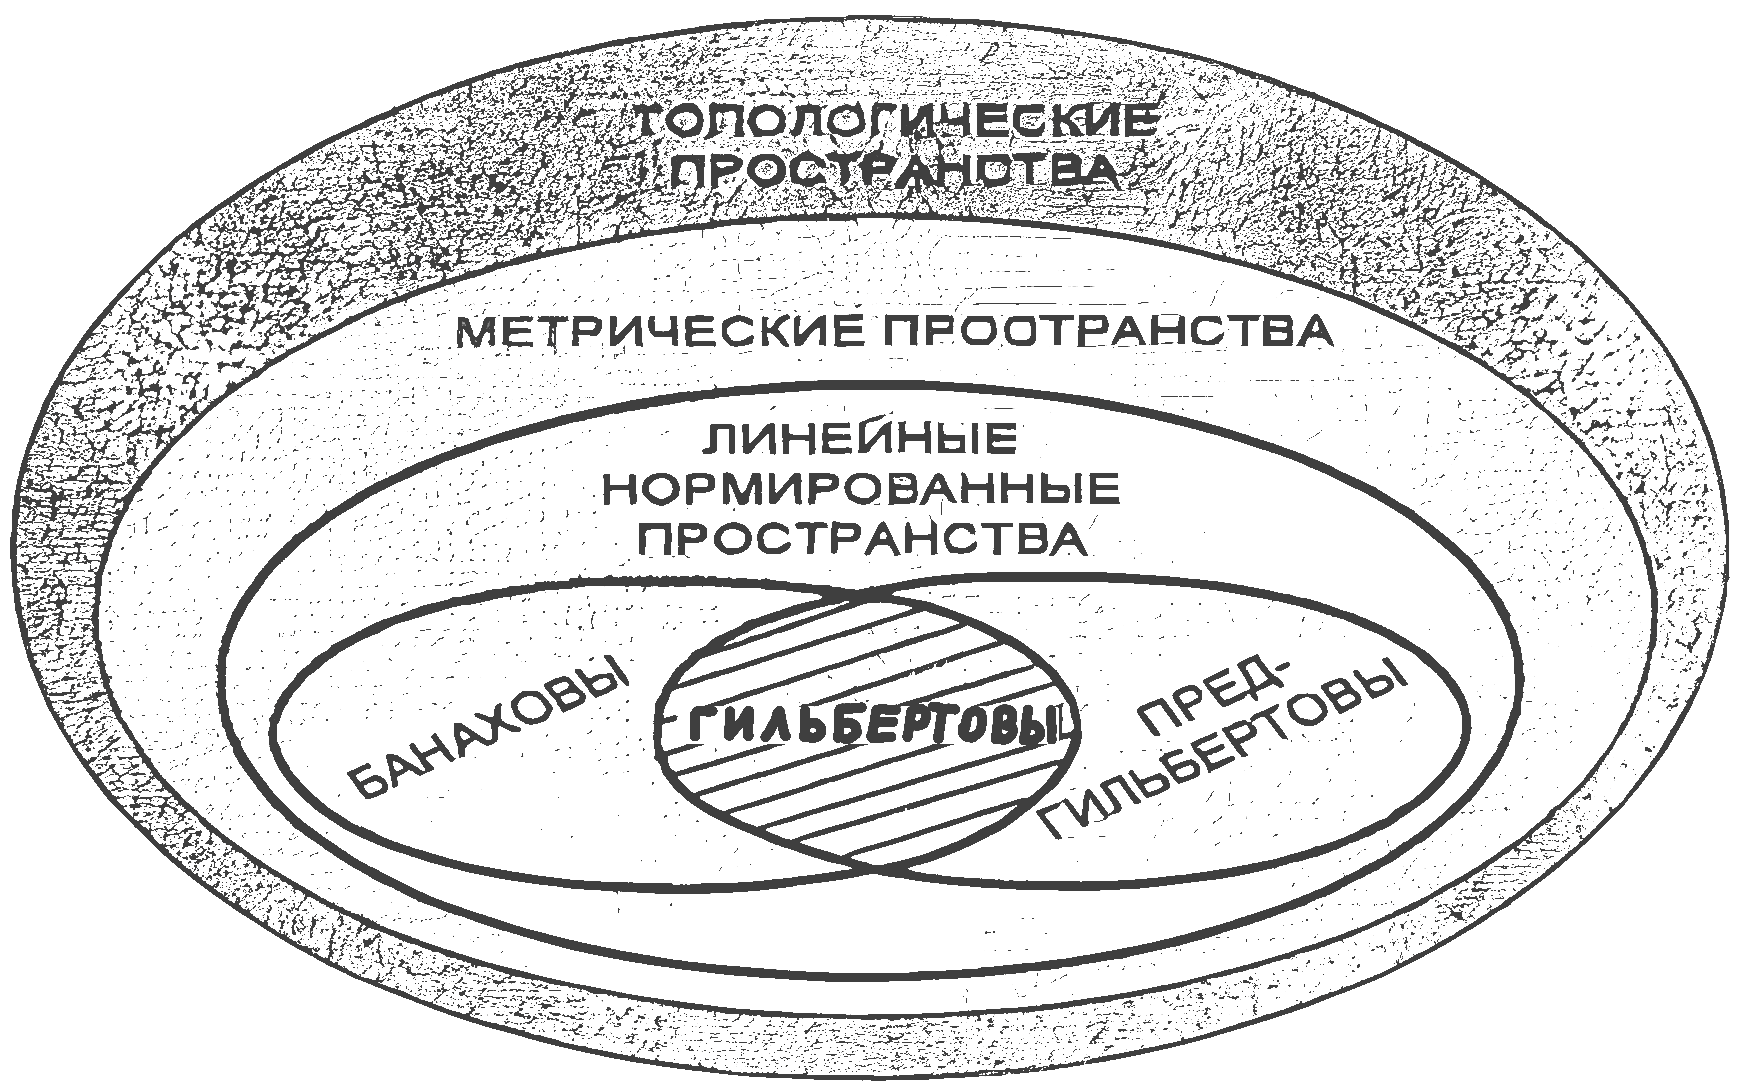
\includegraphics[width=0.5\textwidth]{/Users/vladbelousov/Desktop/Semestr_4-FP-NSU/АМ/Лекции_по_дням/image/1.png}
\end{center}

Кинетическая энергия: \( T = E - U  \) 

\begin{gather*}
    E<U_m : x_1 \le  x \le  x_2 - \text{финитное} \\
    E > Um :- \text{ движение всегда инфинитное}  \\
    E < U_m : x \geq x_3 \text{ - инфинитное} \\
    E = U_m : \\
    \frac{\partial U }{\partial x }(x_m)= 0  \quad  U_x = U_ m + \cancelto{0}{\frac{\partial U}{\partial x }( x_m)}  ( x- x_m) + \frac{1}{2} \frac{ \partial ^2 U }{\partial x ^2}  ( x- x_m ) ^2 + \dots \\
    t-t_0 = -\sqrt{\frac{m}{2} } \int_{ x_0}^{x} \frac{dx}{\sqrt{E- U_m - \frac{1}{2 } U'' (x_m)(x- x_m) ^2 }}= - \sqrt{\frac{m}{- U '' (x_m)} } \int_{ x_0}^{x} \frac{1}{x- x_m} =\\
    = - \sqrt{\frac{m}{- U _{xx} '' (x_m)} } \ln \left| \frac{x- x_m }{x_0 - x_m} \right|  \\   
    \displaystyle  x-x_m = ( x_0- x_m )e^{- \sqrt{\frac{-U''(x_m)}{m} }(t- t_0)} ; \quad  x \xrightarrow{t \to  \infty } x_m 
\end{gather*}

\section{Движение в центральном поле}

\begin{gather*}
    U(\vec{r})\equiv  U ( r)\\
    \vec{F}= - \vec{\nabla }U = - \frac{\partial U}{\partial \vec{r}}= - \frac{\partial U}{\partial \vec{r}} \frac{\vec{r}}{r}    \\
    \vec{M}= [ \vec{r}\times \vec{p }]= \mathrm{const} \\
    \frac{d \vec{M}}{d t }= \underbrace{\left[ \frac{d \vec{ r }} { d t}\times  \vec{p}  \right]}_{\vec{B} \parallel \vec{p}  }    + \underbrace{\left[ \vec{r} \times \frac{d \vec{p}}{d t} \right]}_{\vec{F} \parallel \vec{r} }  =0 \\
    \begin{aligned}
        \begin{cases}
            x= r \cos  \varphi \\    
            y = r \sin  \varphi 
        \end{cases}
        \quad  
    \end{aligned} \\
    \vec{r}= \vec{e_x}x + \vec{e_y}y =  r\cos \varphi \vec{e_x} + r\sin \varphi \vec{e_y} \\  
    \dot{\vec{r}}=\vec{e _ x}( \dot{r} \cos \varphi - \dot{r} \cos  \varphi \dot{\varphi}  ) + \vec{e_y}( \dot{r} \sin \varphi - \dot{r} \sin  \varphi \dot{\varphi}  ) = \\
    =\dot{r}( \cos \varphi \vec{e_x} + \sin \varphi \vec{e_y})+ r \dot{ \varphi}(- \vec{e_x} \sin \varphi + \vec{e_y} \cos \varphi = \dot{r} \vec{e_r}+r \dot{\varphi} \vec{e _{\varphi} } \\
    E = \frac{1}{ 2} m v ^2 + U ( r) = \frac{1}{2 }m ( \dot{ r } ^2+ ( r \dot{\varphi}) ^2  ) + U ( r)     \\
    \vec{M} = [ r \vec{ e_r}\times  m \vec{ v}]= r m \dot{r } \cancelto{0}{[\vec{e_r}\times \vec{e_r}]}+ m r ^2 \dot{\varphi} \underbrace{[\vec{e_r}\times  \vec{ e _{\varphi} }]}_{\vec{e_z}}  \\
    \vec{M}=\begin{pmatrix}
    0\\
    0\\
    M
    \end{pmatrix} \Rightarrow M = m r ^2 \dot{\varphi}  \Rightarrow d \varphi = \frac{M}{m r ^2 } dt  \quad  (1)
\end{gather*}

\begin{gather*}
    E = \frac{1}{ 2 } m \dot{r} ^2 +  \underbrace{U(r) + \frac{M ^2}{2 mr ^2 }}_{U_{\text{эф}}}     \\
    t-t_0 = \pm  \sqrt{\frac{m}{2} } \int_{ r_0}^{r}   \frac{dr}{\sqrt{E - U _{\text{эф}}(r) }} \overset{(1)}{\Rightarrow }   \varphi - \varphi_0 - \pm \frac{M}{\sqrt{2m}} \int_{r_0}^{r} \frac{dr}{r ^2 \sqrt{E - U _{\text{эф}}(r) }}   
\end{gather*}

\section{Секторальная скорость}

\begin{center}
    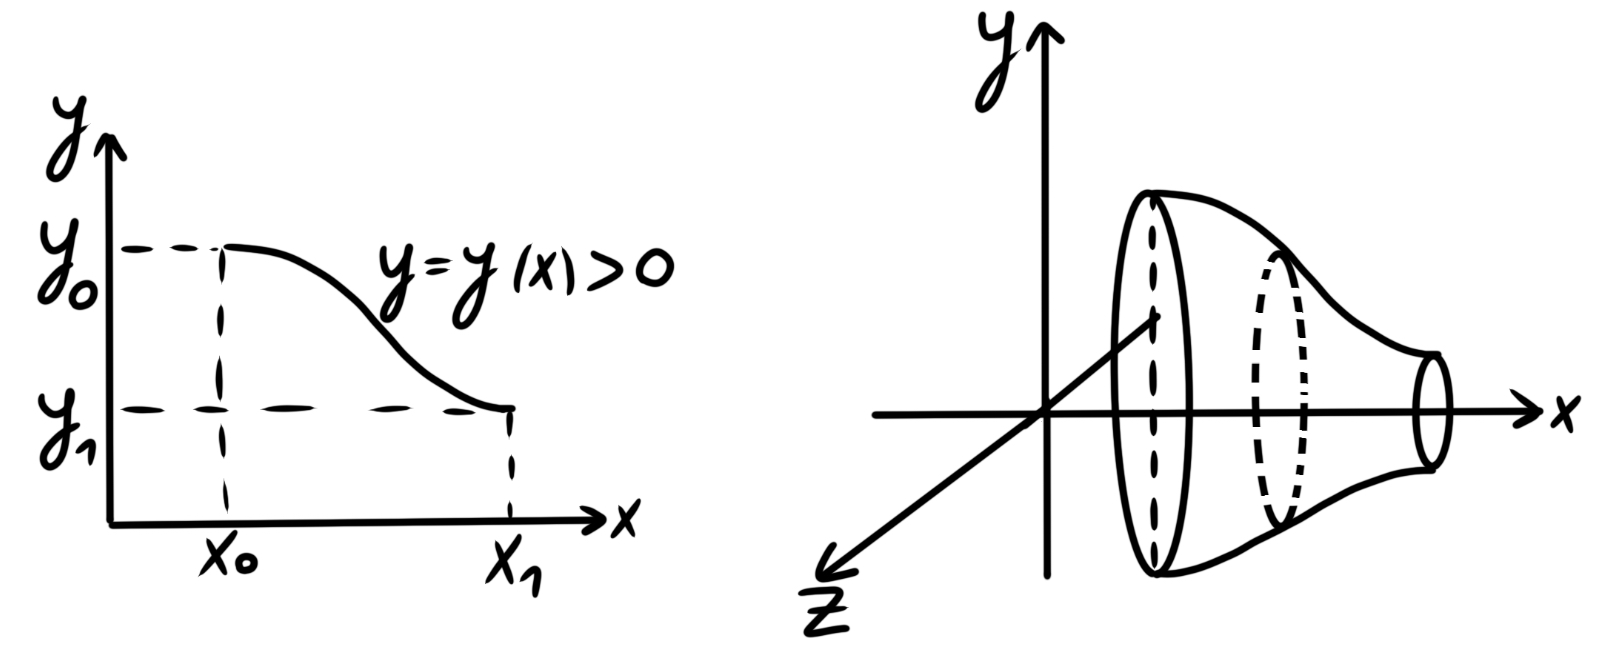
\includegraphics[width=0.35\textwidth]{/Users/vladbelousov/Desktop/Semestr_4-FP-NSU/АМ/Лекции_по_дням/image/2.png}
\end{center}

    \[ \frac{ds }{dt}  = \frac{\frac{1}{2} r r d \varphi }{dt} = \frac{M}{2m} = \mathrm{const}               \] 

Задача Кеплера: 

\begin{center}
    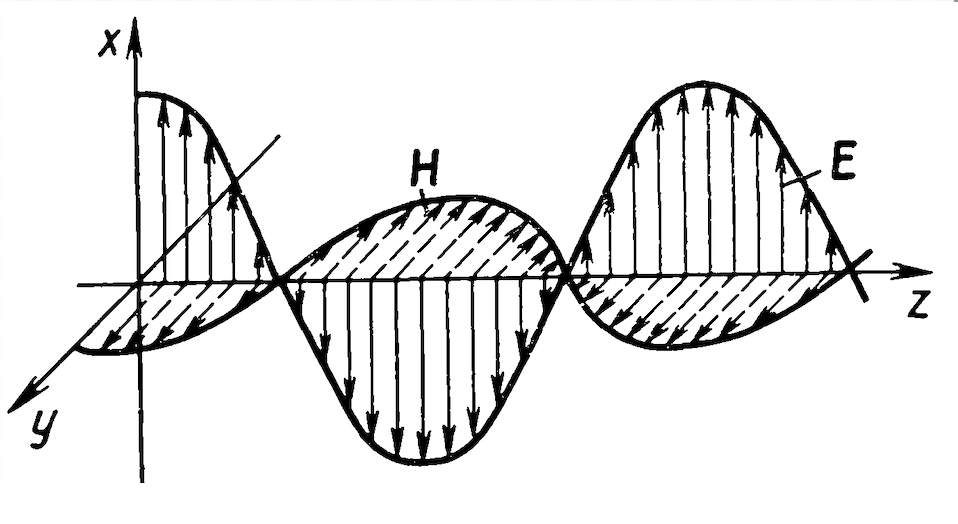
\includegraphics[width=0.5\textwidth]{/Users/vladbelousov/Desktop/Semestr_4-FP-NSU/АМ/Лекции_по_дням/image/3.png}
\end{center}

    \[ E \geq 0 - \text{инфинитное}  \quad  E < 0 - \text{инфинитное}  \] 

\[ U = -\frac{\alpha}{r} \quad  U _{\text{эф} } = - \frac{\alpha}{r} + \frac{M ^2 }{2 mr ^2 }    \] 

\[ \begin{aligned}
    \begin{array}{l}
        \displaystyle \varphi - \varphi_0 = \pm  \frac{M}{\sqrt{2m}} \int_{ r_0}^{r}  \frac{dr}{ r ^2 \sqrt{E + \frac{\alpha}{ r} - \frac{M ^2 }{2mr ^2 }  }} \\
        U = \frac{p}{ r}, \text{ где p параметр орбиты : }   p = \frac{M ^2 }{m \alpha} \\
        e = \sqrt{ 1 + \frac{2E M ^2 }{m \alpha ^2} } \text{ - эксцентриситет} \\
    \end{array}
    \quad  \Rightarrow \varphi - \varphi_0 = \pm  \int  \frac{dU}{\sqrt{ e ^2 - ( u -1 ) ^2 }}= \arccos {\frac{u-1}{e} } \\ 
\end{aligned}  \] 

\begin{center}
    \[ r= \frac{p}{1 + r \cos  ( \varphi - \varphi_0)} \] 

\( e>1 ( E >0) \) - гипербола 

\( e=1  ( E=0) \) - парабола

\( e<1 ( E<0) \) - эллипс 

\( e = 0 ( E = - \frac{m\alpha} {2 M ^2} ) \) - окружность
\end{center}


%%-------------------------------%%

% Закрытие документа, если файл компилируется отдельно
\ifdefined\mainfile
    % Если это основной файл, не нужно заканчивать документ
\else
    \end{document}
\fi